\documentclass[a4paper, 12pt]{article}

\usepackage{fontspec}
\usepackage{polyglossia}
\defaultfontfeatures{Ligatures=TeX}
\setdefaultlanguage{russian}
\setotherlanguage{english}
\setmainfont{Times New Roman}
\newfontfamily{\latinfont}{Times New Roman}
\newfontfamily{\cyrillicfont}{Times New Roman}
\newfontfamily{\cyrillicfonttt}{Courier New}

\usepackage{geometry}
\usepackage{amsmath}
\usepackage{amssymb}
\usepackage{amsfonts}
\usepackage{graphicx}
\usepackage{float}
\usepackage{wrapfig}
\usepackage{subcaption}
%\usepackage[caption=false]{subfig}
\geometry{right=20mm}
\geometry{left=20mm}
\geometry{top=20mm}
\geometry{bottom=20mm}

\usepackage{indentfirst}
\usepackage[outputdir=auxiliary]{minted}

\graphicspath{{../img/}}
\DeclareMathOperator{\R}{\mathbb{R}}
\DeclareMathOperator{\C}{\mathbb{C}}
\renewcommand{\Re}{\mathrm{Re}}
\renewcommand{\Im}{\mathrm{Im}}


\DeclareMathOperator{\sign}{sgn}

\begin{document}
    \begin{titlepage}
    \begin{center}
        \textit{МИНИСТЕРСТВО ОБРАЗОВАНИЯ И НАУКИ\\
        РОССИЙСКОЙ ФЕДЕРАЦИИ}
        \vspace{1ex}

        федеральное государственное бюджетное образовательное учреждение\\
        высшего профессионального образования
        \vspace{1ex}

        \textbf{САНКТ-ПЕТЕРБУРГСКИЙ НАЦИОНАЛЬНЫЙ ИССЛЕДОВАТЕЛЬСКИЙ УНИВЕРСИТЕТ ИТМО}
        \vspace{13ex}

        Лабораторная работа №3\\
        <<Динамика нелинейных систем>>\\
        по дисциплине <<Моделирование технических систем>>\\
        \vspace{1em}
        Вариант 3\\
    \end{center}
    \vspace{14em}
    \begin{flushright}
        \noindent
        Выполнили:\\
        студенты гр. R4133c\\
        Борисов М. В.\\
        Симонов П.\\
        Мацуганов А. И.\\
        \vspace{1em}
        Преподаватель:\\
        Семенов Д. М.
    \end{flushright}
    \vfill
    \begin{center}
        \large{Санкт-Петербург}\\
        2021 г.\\
    \end{center}
\end{titlepage}

    \setcounter{page}{2}
    \setlength{\parindent}{0pt}

    \section*{Задание}
    Дана система с постоянной задержкой $h$
    \begin{equation}
        \label{z_sys}
        \dot{x}(t) = Ax(t) + A_1 x(t- h), \, \mbox{где } x \in \R^2
    \end{equation}

    \begin{equation*}
        A =
        \begin{pmatrix}
            3& 1\\
            2& 2
        \end{pmatrix}
        ,\,A_1 =
        \begin{pmatrix}
            -5& 1\\
            -2& -4
        \end{pmatrix}
    \end{equation*}

    \begin{enumerate}
        \item Промоделировать данную систему
        \item Используя дескрипторный метод, найти максимальную задержку, при которой данная система будет устойчивой.
        \item Построить регулятор $u(t) = Kx(t)$ такой, чтобы замкнутая система \[\dot{x}̇(t) = Ax(t) + A_1x(t − h) + Iu(t) = (A + K)x(t) + A_1x(t − h)\] была устойчивой при любых задержках $h$.
    \end{enumerate}

    \subsection*{Решение}

    Промоделируем систему с различными $h$
    \begin{figure}[H]
        \centering
        \begin{subfigure}{0.49\linewidth}
            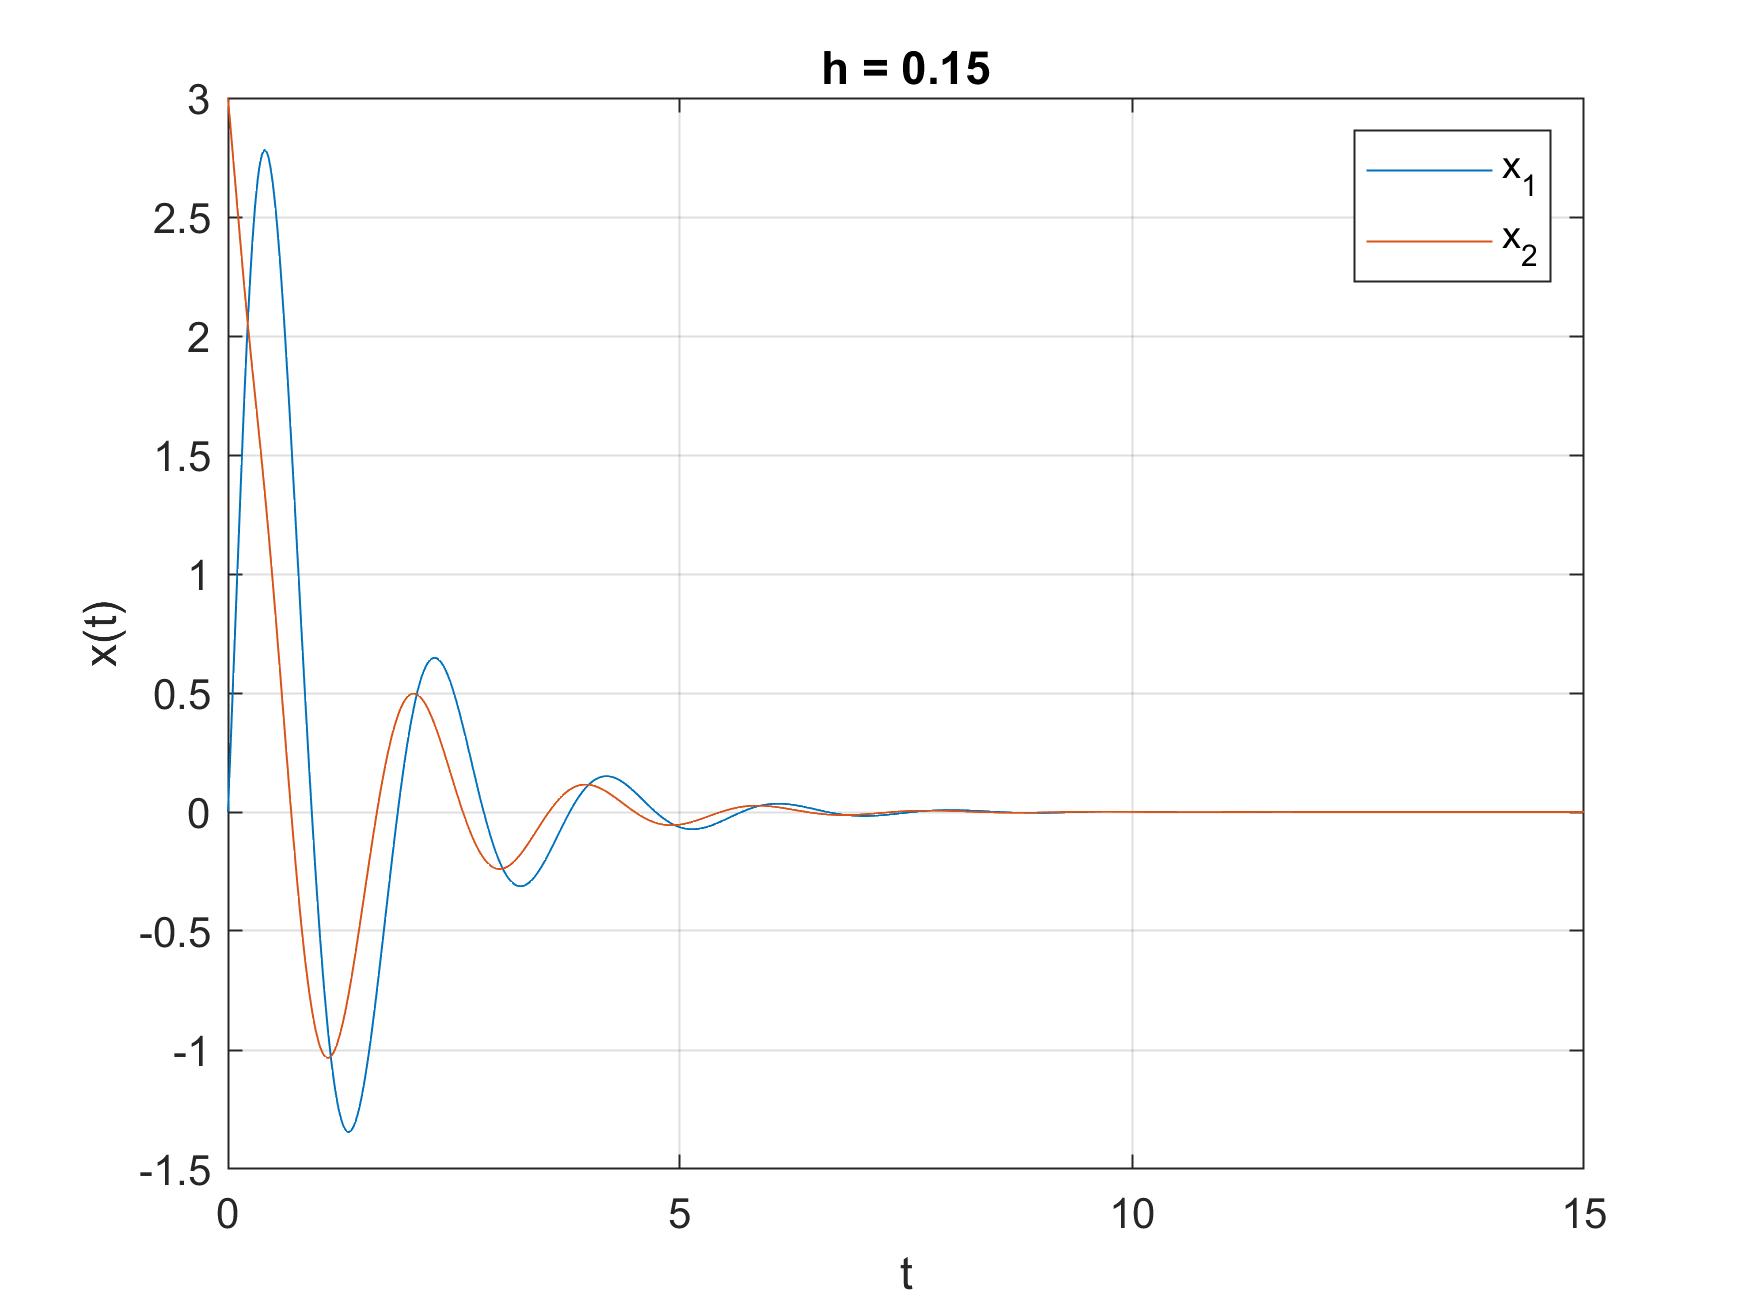
\includegraphics[width=\linewidth]{L6h0.15.png}
            \caption{Устойчивый случай}
        \end{subfigure}
        \begin{subfigure}{0.49\linewidth}
            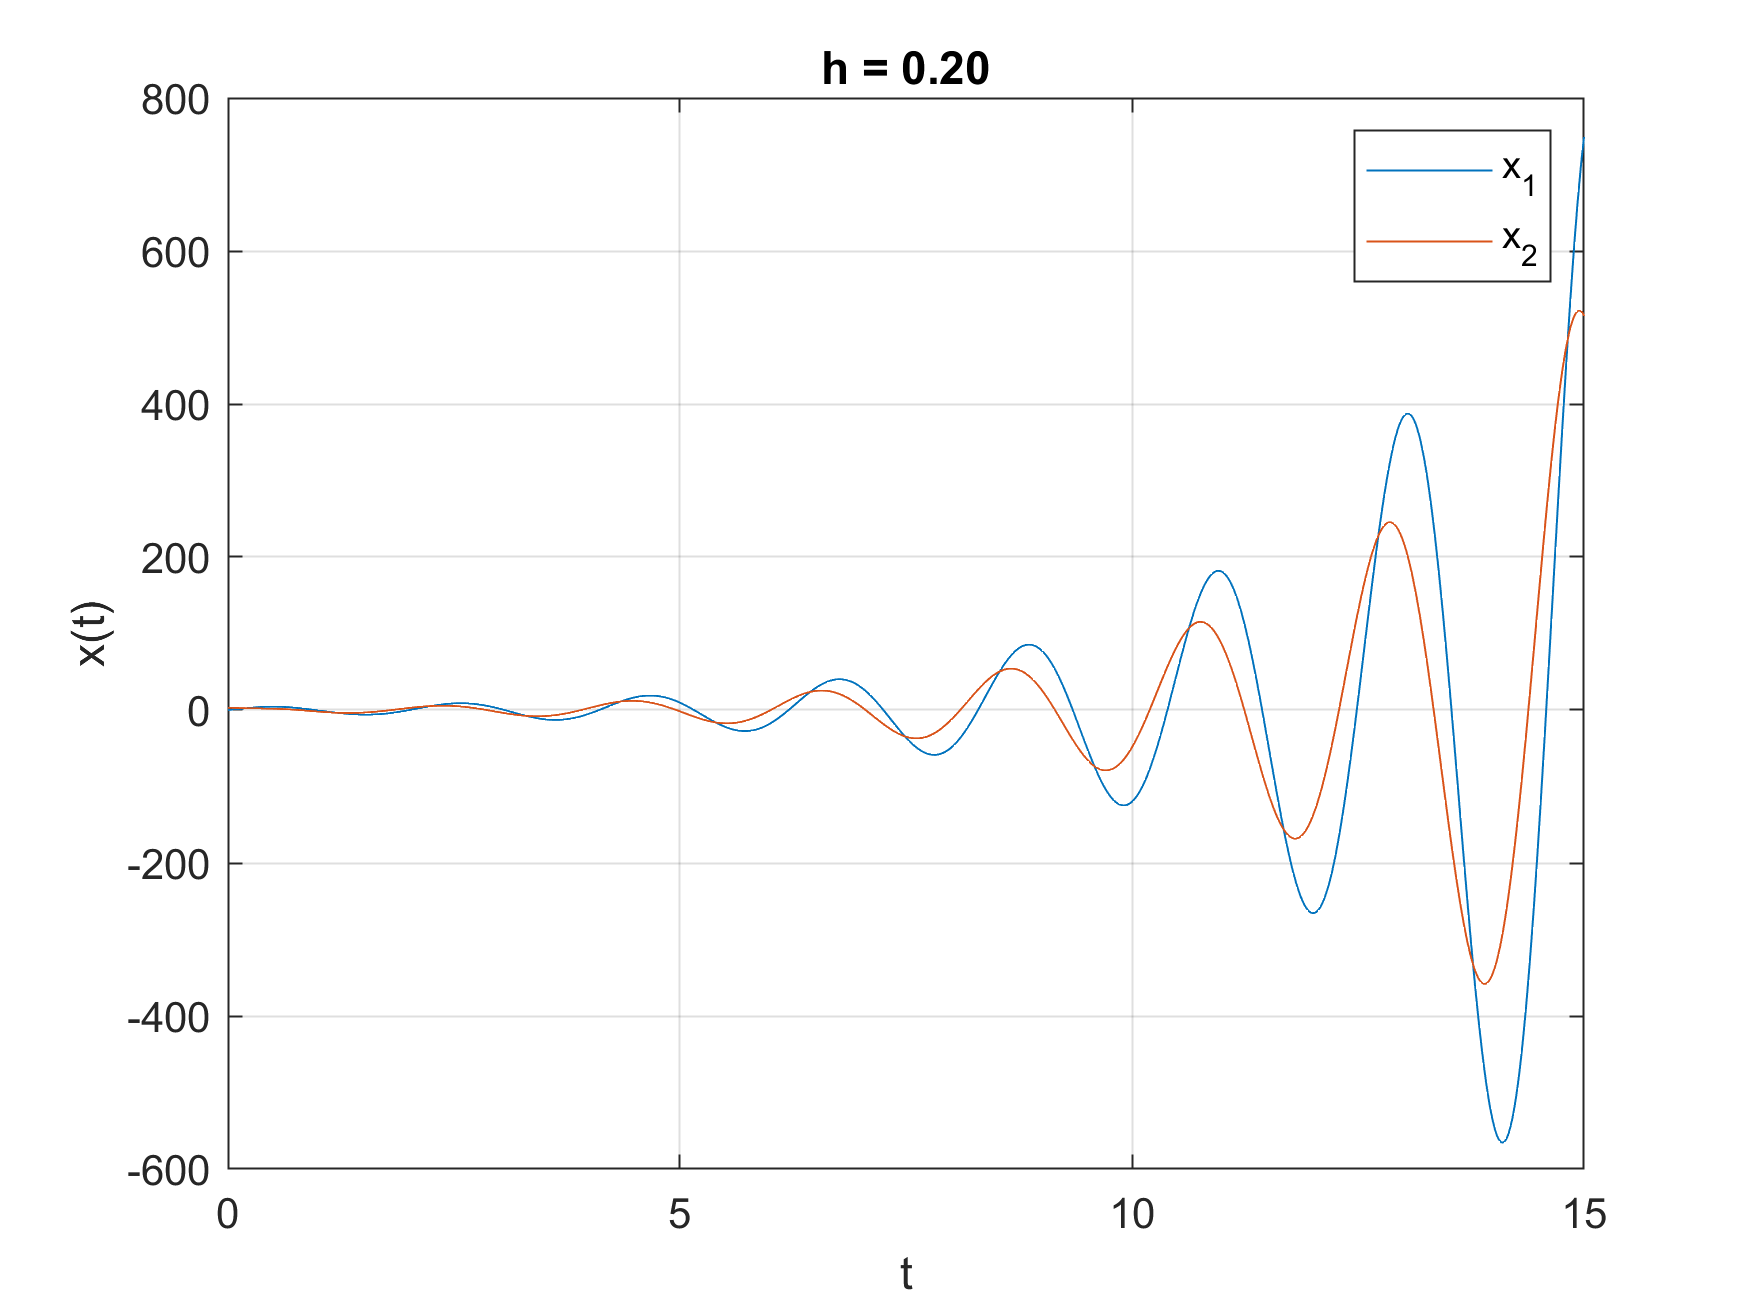
\includegraphics[width=\linewidth]{L6h0.20.png}
            \caption{Неустойчивый случай}
        \end{subfigure}
        \caption{Моделирование системы~\eqref{z_sys}}
    \end{figure}


    Используя дескрипторный метод, найдем
    максимальную задержку h, при которой исследуемая система будет
    устойчивой. Для этого необходимо решить следующую систему
    линейных матричных неравенств:

    \begin{equation}
        \psi =
        \begin{bmatrix}
            P_2^T(A + A_1) + (A + A_1)^T P_2 & P - P_2^T + (A + A_1)^T P_3 & -hP_2^T A_1\\
            * & -P_3 - P_3^T + hR & -hP_3^T A_1\\
            * & * & -hR
        \end{bmatrix}
        < 0,
    \end{equation}
    \[P>0,\,R>0\]
    В результате решения неравенства получена максимальная задержка $h = 0.18$, при которой система является устойчивой.
    \begin{figure}[H]
        \centering
        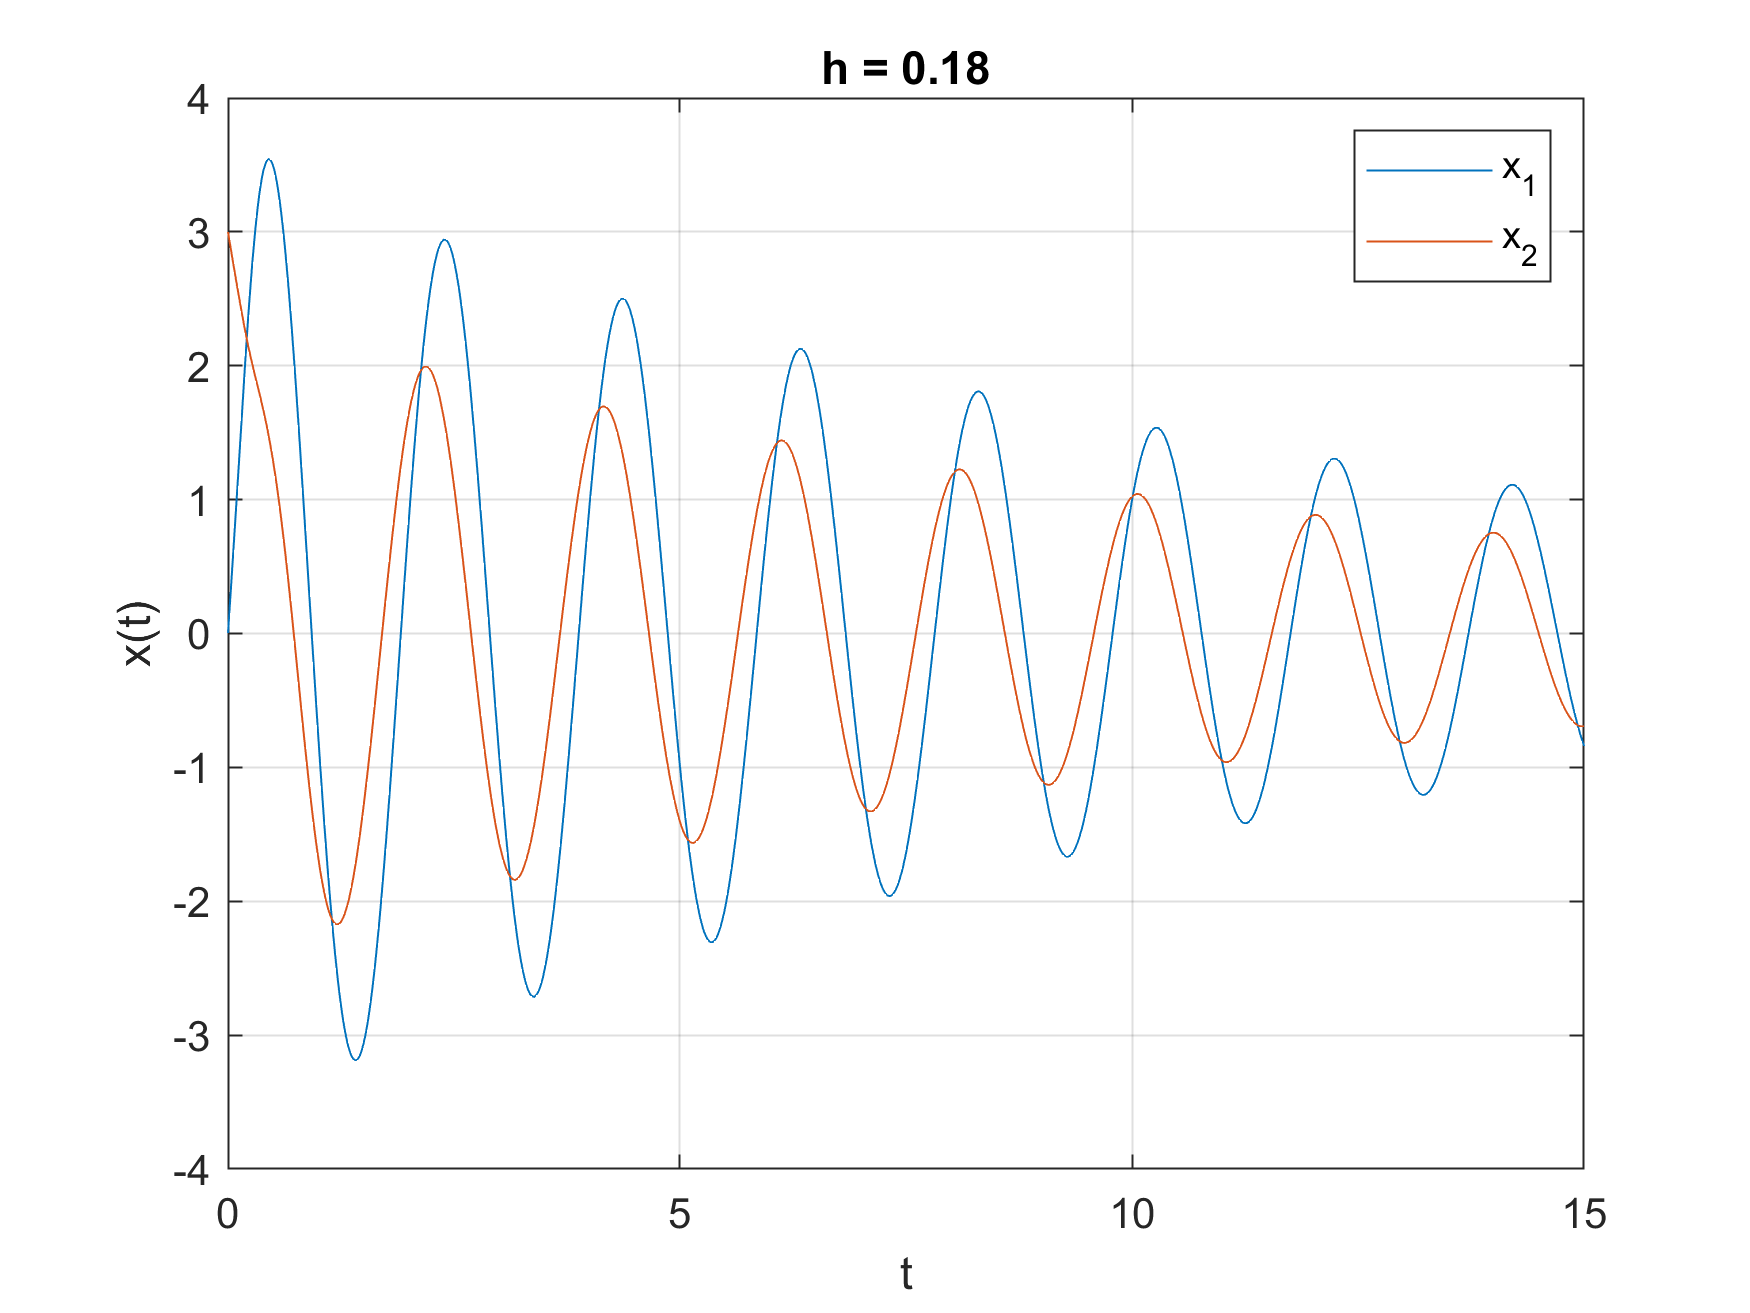
\includegraphics[width=0.75\linewidth]{L6h0.18.png}
        \caption{Моделирование системы~\eqref{z_sys} при максимальной задержке}
    \end{figure}

    Используя метод Ляпунова-Красовского,
    найдем такое $K$ для регулятора $u(t) = Kx(t)$, чтобы замкнутая
    система была устойчива. Для этого достаточно решить матричное
    неравенство:
    \begin{equation}
        \psi =
        \begin{bmatrix}
            \tilde{A}^T P + P\tilde{A} + Q & PA_{1}\\
            A_{1}^TP & -Q
        \end{bmatrix}
    \end{equation} где $P = P^T>0,\,Q=Q^T>0,\,\tilde{A}=A+K$

    Получаем матричный коэффициент $K$:
    \begin{equation}
        K =
        \begin{bmatrix}
            -35.4556 & -17.4925\\
            -18.4925 & -25.2699
        \end{bmatrix}
    \end{equation}

    Промоделируем систему с различными $h$
    \begin{figure}[H]
        \centering
        \begin{subfigure}{0.49\linewidth}
            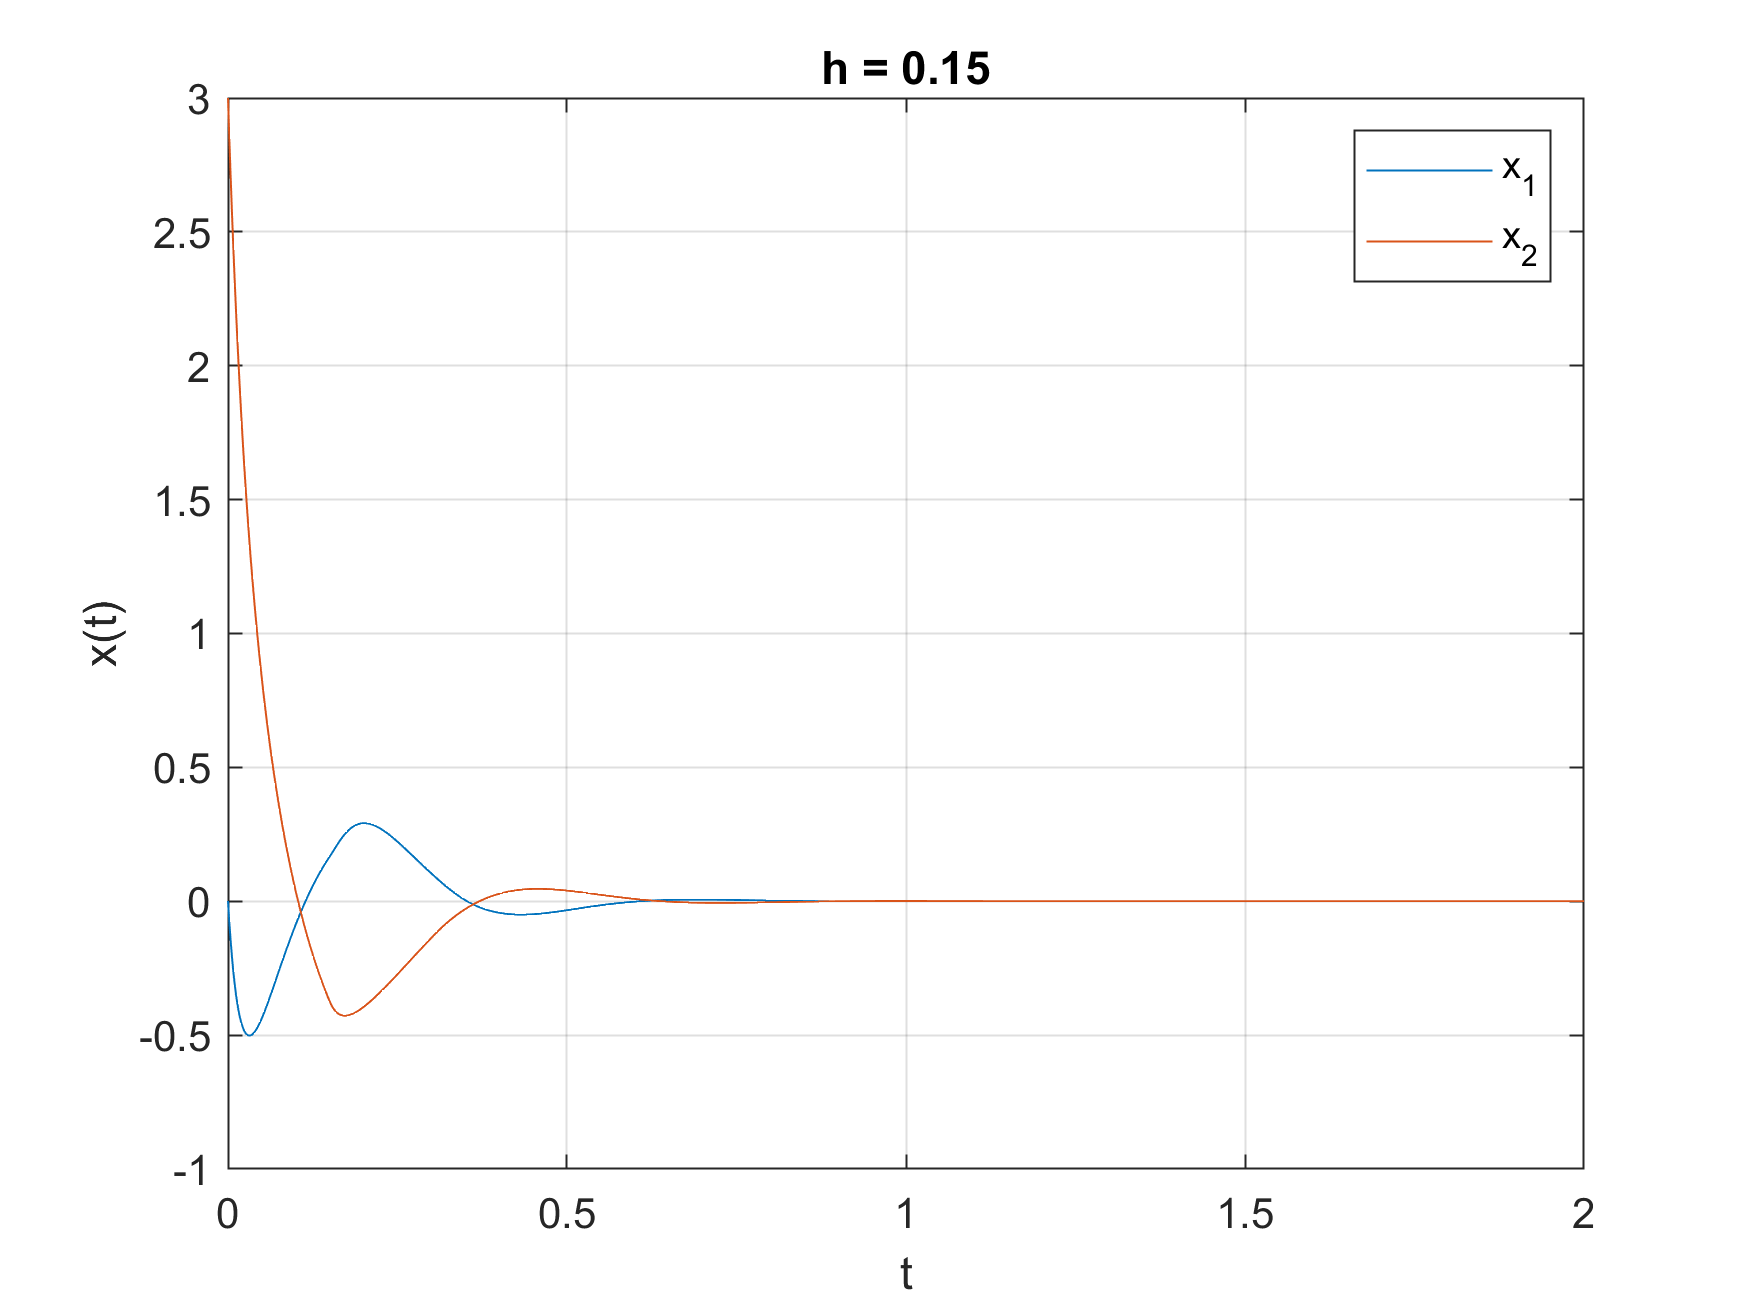
\includegraphics[width=\linewidth]{L62h0.15.png}
            \caption{Устойчивый случай}
        \end{subfigure}
        \begin{subfigure}{0.49\linewidth}
            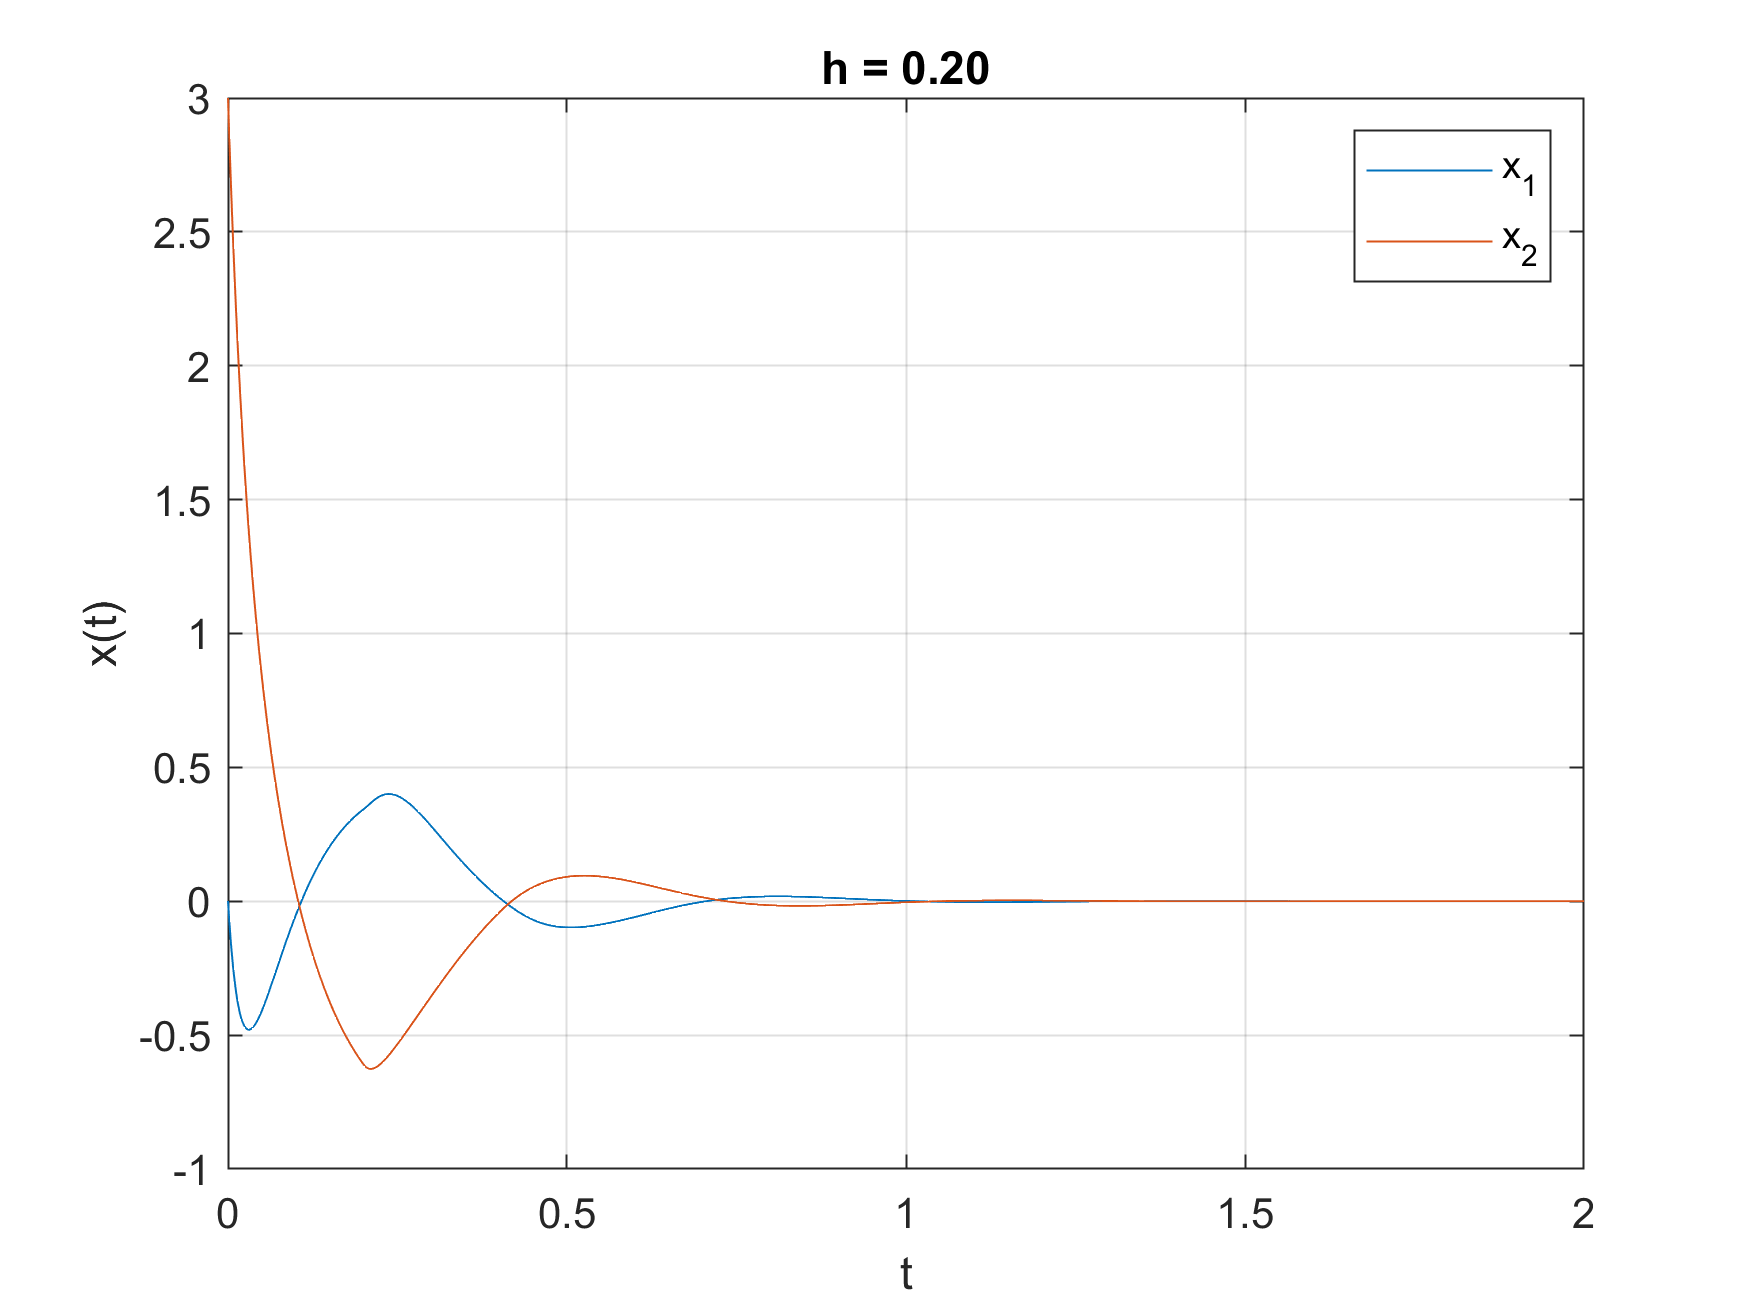
\includegraphics[width=\linewidth]{L62h0.20.png}
            \caption{Неустойчивый случай}
        \end{subfigure}
        \begin{subfigure}{0.49\linewidth}
            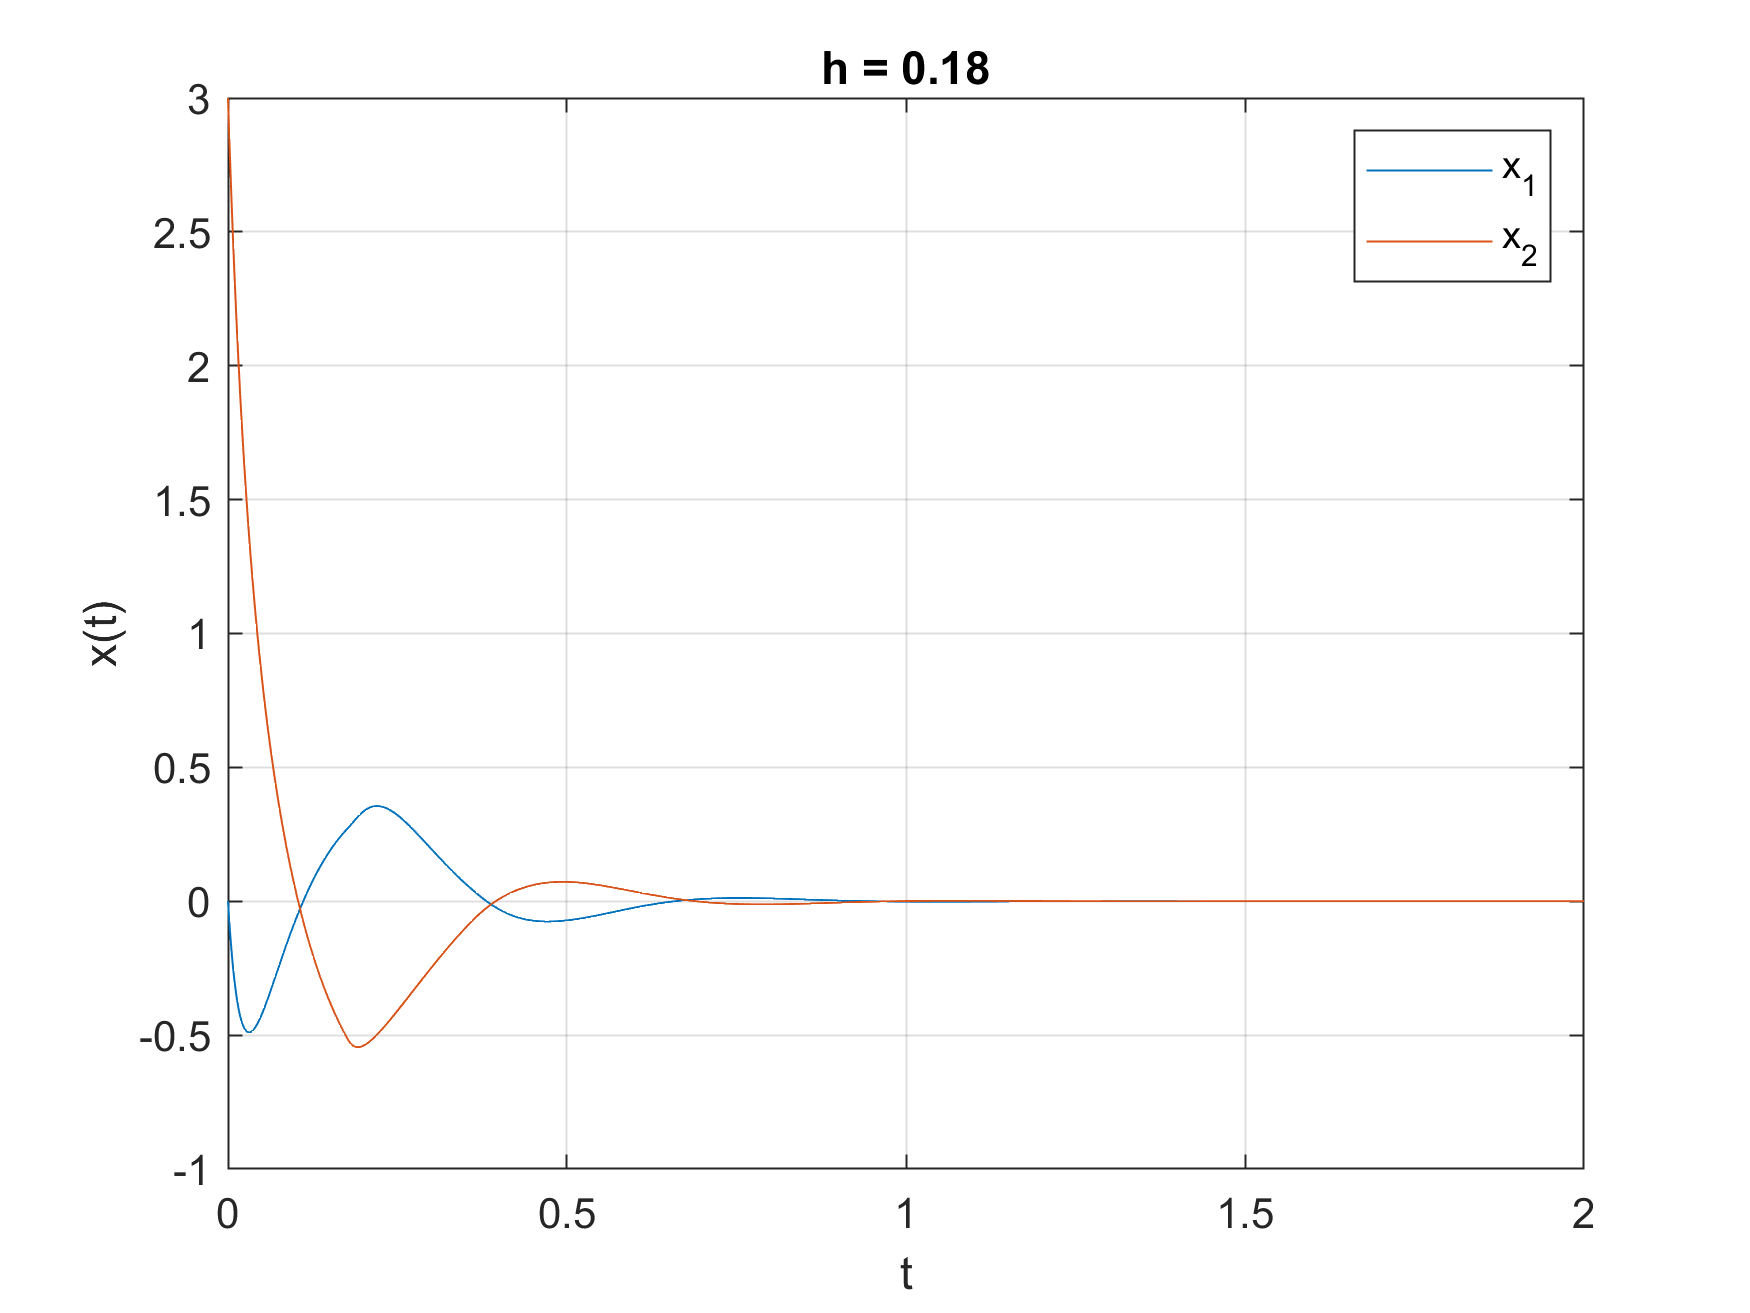
\includegraphics[width=\linewidth]{L62h0.18.png}
            \caption{Максимальная задержка}
        \end{subfigure}
        \caption{Моделирование замкнутой системы}
    \end{figure}
    \section*{Вывод}
    В данной работе был исследован дескрипторный метод с помощью которого была установлена максимально возможная задержка
    незамкнутой системы с произвольной постоянной задержкой. Изучен метод построения регулятора для замкнутой системы с
    целью стабилизации системы при любой задержке.
\end{document}
